
\section{Evaluation}
	\label{sec:eval}
The evaluation procedure focuses on identifying a person from the footprints of individual steps. 
As shown in Fig. \ref{fig:step_frames}, the steps are present in sequences of the pressure mapping imageries of individual steps, which we use as the original dataset. The dataset includes overall 529 sequences from 13 participants. 

In our previous work \cite{blind}, a fast wavelet transform is applied to these sequences of steps to generate a single 336 dimension wavelet descriptor for each step. These features are then classified using a support vector machine classifier with a quadratic kernel \cite{cortes1995support}. This approach results in a classification accuracy of 76.9\%.
Our approach diverges after the steps are segmented and the flowchart for our proposed approach can be seen in Fig. \ref{fig:flowchart}. We generate the dataset of images which are maximum frame (sum of all pixels per frame), average frame (average of all the frames present in a sequence) and the set of all the frames forming a step; after that this set of images is passed through the pre-trained Inception model, for feature extraction, which upon classification gives the recognition results for person identification.

\subsubsection{Maximum Frames}
As described in Section \ref{sec:mod}, the maximum frame corresponds to the point at which the foot exerts maximum pressure on the ground. The pressure mat scans at the rate of 25 fps, thus a single frame corresponds to the information captured in 40 milliseconds. Our assumption is that the maximum frame of each step corresponds to the situation when a person's entire foot is on the ground, and hence, contains enough spatial information to be discriminative. 
\par
We evaluate our system by using these images for all the steps present in our dataset. These images are passed through the pre-trained Inception model and the activations of the fully-connected layer are used as image descriptors. To complete the classification task, the image descriptors are fed to a fully-connected layer, which computes the probability distribution over the different classes using \emph{softmax} activation function. The schematic diagram of the architecture followed for this approach is shown in Fig. \ref{fig:ann_pipeline}. This entire process is carried out with a 10-fold cross validation and repeated for 10 iterations. We calculate the average of the result obtained after each repetition. The final recognition rate after this method comes out to be 71.99\% as shown in Table \ref{tab:results}. 

\begin{table}[!t]
	\renewcommand{\arraystretch}{1.3}
	\caption{Person identification accuracies for different image sets and feature types.}
	\label{tab:results}
	\centering
	\begin{tabular}{|c|c|c|}
		\hline
		\bfseries Feature Type & \bfseries Image Set Type & \bfseries Accuracy \\
		\hline
		Wavelet Transformation & All sequences in a step & 76.9\%\\
		\hline
		Deep CNN & Maximum frame & 71.99\%\\
		\hline
		Deep CNN & Average frame & 78.41\%\\
		\hline
		Deep CNN + RNN & Complete step sequence & \bfseries87.66\%\\
		\hline
	\end{tabular}
\end{table}

\subsubsection{Average Frames}
The walking pattern of a person has a temporal component within it. This time dimension includes the way a person starts with engaging his/her foot on the floor, which begins with the heel strike and then carries on until the toe off. Within these stages, the way an individual exerts pressure on the floor varies from person to person. In order to accommodate this temporal information, we average over all the frames in the sequence of a single step and compute images corresponding to all the steps. The evaluation is carried out in the similar manner as with the maximum frames (as seen in Fig. \ref{fig:ann_pipeline}) with a $10 \times 10$ cross-validation and the average recognition rate is 78.41\% as seen in Table \ref{tab:results}. 



\subsubsection{Image Sequences with Recurrent Neural Network}

 In our experiments with the maximum and average frames, we observe that the average frames show an improvement over the  maximum frames. Even though the classification accuracy is improved by the information encoded in the average frames, a certain amount of information is lost by the averaging procedure. Hence, we experiment with using a RNN to classify the temporal sequence of each step. As shown in Fig.  \ref{fig:rnn_pipeline}, all of frames associated with a step are processed through the Inception-v3 model to extract a single descriptor for each frame. 
These descriptors are then fed one after another into a layer of Gated Recurrent Units (GRU) \cite{cho2014properties}, which generates a classification upon completing the sequence. We follow the same evaluation procedure outlined in the previous experiments and we obtain a classification accuracy of 87.66\% (Table \ref{tab:results}).


\begin{figure}
	\centering
		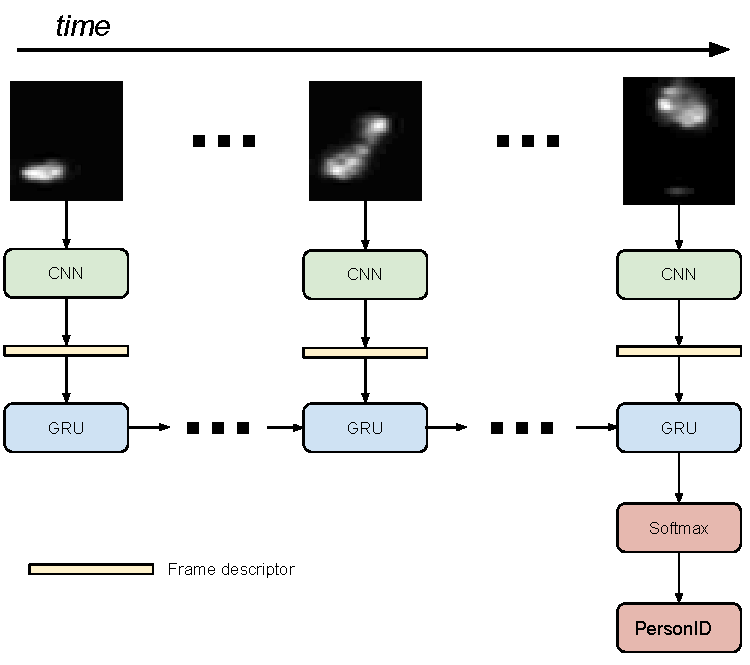
\includegraphics[width=6cm]{./figures/rnn_pipeline.pdf}
	\caption{Schematic diagram of all frames in a single step classification pipeline.}
	\label{fig:rnn_pipeline}
\end{figure}

